% !TEX program = pdflatex
\documentclass[aspectratio=169, 10pt]{beamer}

% ── Theme & colours ──────────────────────────────────────────────────────────
\usetheme{Madrid}
\usecolortheme{default}
\definecolor{primaryblue}{RGB}{0,84,147}
\setbeamercolor{structure}{fg=primaryblue}
\setbeamercolor{title}{fg=white, bg=primaryblue}
\setbeamercolor{frametitle}{fg=white, bg=primaryblue}
\setbeamertemplate{navigation symbols}{}          % remove navigation buttons
\setbeamertemplate{footline}{                      % custom footer
  \leavevmode\hbox{%
    \begin{beamercolorbox}[wd=.33\paperwidth,ht=2.5ex,dp=1.1ex,center]{author in head/foot}%
      \usebeamerfont{author in head/foot}\insertshortauthor
    \end{beamercolorbox}%
    \begin{beamercolorbox}[wd=.34\paperwidth,ht=2.5ex,dp=1.1ex,center]{title in head/foot}%
      \usebeamerfont{title in head/foot}\insertshorttitle
    \end{beamercolorbox}%
    \begin{beamercolorbox}[wd=.33\paperwidth,ht=2.5ex,dp=1.1ex,right]{date in head/foot}%
      \usebeamerfont{date in head/foot}\insertframenumber{} / \inserttotalframenumber\hspace*{2ex}
    \end{beamercolorbox}}%
  \vskip0pt%
}

% ── Packages ─────────────────────────────────────────────────────────────────
\usepackage[utf8]{inputenc}
\usepackage[T1]{fontenc}
\usepackage{booktabs}
\usepackage{graphicx}
\usepackage{xcolor}
\usepackage{tikz}
\usepackage{hyperref}
\usepackage{bookmark}
\usepackage{listings}

\lstset{
  basicstyle=\ttfamily\scriptsize,
  keywordstyle=\color{primaryblue}\bfseries,
  commentstyle=\color{gray},
  breaklines=true,
  frame=single,
  rulecolor=\color{gray!30},
  backgroundcolor=\color{gray!5},
}

% ── Title ────────────────────────────────────────────────────────────────────
\title[Health Insurance Cross-Sell]{Health Insurance Cross-Sell Prediction}
\subtitle{Machine Learning Project Work}
\author{Giacomo Piergentili}
\date{2025/2026}

% ══════════════════════════════════════════════════════════════════════════════
\begin{document}

% ── Slide 1: Title ───────────────────────────────────────────────────────────
\begin{frame}
  \titlepage
\end{frame}

% ══════════════════════════════════════════════════════════════════════════════
\section{Introduction}
% ══════════════════════════════════════════════════════════════════════════════

% ── Slide 2: Problem Statement ──────────────────────────────────────────────
\begin{frame}{Problem Statement}
  \begin{block}{Business context}
    An insurance company wants to identify its \textbf{health insurance} customers
    who are also likely to purchase \textbf{vehicle insurance}.
  \end{block}

  \vspace{0.4cm}
  \begin{itemize}
    \item \textbf{Goal:} predict whether a customer will respond positively to a
          cross-sell offer (\texttt{Response} $\in \{0, 1\}$)
    \item \textbf{Metric:} ROC-AUC
    \item \textbf{Dataset:} $\sim$11.5\,M labelled customer records
    \item \textbf{Source:} Kaggle Playground Series, Season 4, Episode 7
  \end{itemize}

  \vspace{0.3cm}
  \footnotesize
  Original dataset: \textit{Health Insurance Cross Sell Prediction} by Anmol Kumar (Kaggle).
\end{frame}

% ── Slide 3: Project Pipeline ───────────────────────────────────────────────
\begin{frame}{Project Pipeline}
  \begin{center}
    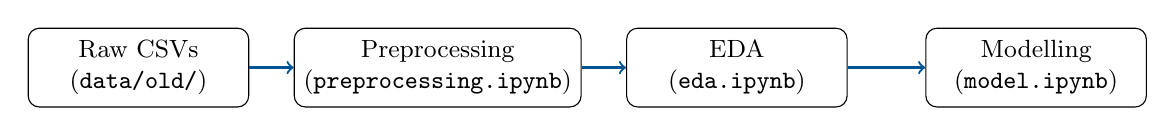
\begin{tikzpicture}[
      node distance=1.8cm,
      every node/.style={draw, rounded corners, minimum height=1cm,
                         minimum width=2.8cm, align=center, font=\small},
      arrow/.style={->, thick, primaryblue}
    ]
      \node (raw)   {Raw CSVs\\(\texttt{data/old/})};
      \node (prep)  [right of=raw, xshift=2cm] {Preprocessing\\(\texttt{preprocessing.ipynb})};
      \node (eda)   [right of=prep, xshift=2cm] {EDA\\(\texttt{eda.ipynb})};
      \node (model) [right of=eda, xshift=2cm] {Modelling\\(\texttt{model.ipynb})};
      \draw[arrow] (raw)  -- (prep);
      \draw[arrow] (prep) -- (eda);
      \draw[arrow] (eda)  -- (model);
    \end{tikzpicture}
  \end{center}

  \vspace{0.5cm}
  \begin{itemize}
    \item All intermediate data stored as \textbf{Parquet} files (columnar, compressed, dtype-preserving)
    \item Reproducible: each notebook reads the output of the previous one
  \end{itemize}
\end{frame}

% ── Slide 4: Dataset Overview ────────────────────────────────────────────────
\begin{frame}{Dataset Overview}
  \begin{table}[h]
    \centering
    \small
    \begin{tabular}{@{}llp{6.5cm}@{}}
      \toprule
      \textbf{Feature} & \textbf{Type} & \textbf{Description} \\
      \midrule
      \texttt{Age}                  & int   & Customer age (20--85) \\
      \texttt{Gender}               & cat   & Male / Female \\
      \texttt{Driving\_License}     & bin   & 1 = holds a licence \\
      \texttt{Region\_Code}         & cat   & 53 distinct regions (0--52) \\
      \texttt{Previously\_Insured}  & bin   & 1 = already has vehicle insurance \\
      \texttt{Vehicle\_Age}         & ord   & $<$1 yr / 1--2 yr / $>$2 yr \\
      \texttt{Vehicle\_Damage}      & bin   & 1 = vehicle was previously damaged \\
      \texttt{Annual\_Premium}      & int   & Amount paid for health insurance \\
      \texttt{Policy\_Sales\_Channel} & cat & 152 distinct sales channels \\
      \texttt{Vintage}              & int   & Days since the customer joined \\
      \texttt{Response}             & bin   & \textbf{Target}: 1 = interested \\
      \bottomrule
    \end{tabular}
  \end{table}
\end{frame}

% ══════════════════════════════════════════════════════════════════════════════
\section{Data Preprocessing}
% ══════════════════════════════════════════════════════════════════════════════

% ── Slide 5: Data Inspection & Encoding ──────────────────────────────────────
\begin{frame}{Data Inspection \& Encoding}
  \begin{columns}[T]
    \begin{column}{0.48\textwidth}
      \textbf{Quick checks}
      \begin{itemize}
        \item $\sim$11.5\,M rows $\times$ 12 columns
        \item No missing values, no duplicates
        \item 3 columns stored as strings that need encoding
      \end{itemize}

      \vspace{0.3cm}
      \textbf{Problems found}
      \begin{itemize}
        \item \texttt{Gender}, \texttt{Vehicle\_Age}, \texttt{Vehicle\_Damage} stored as strings
        \item Most numeric columns use \texttt{int64}/\texttt{float64} (way bigger than needed)
      \end{itemize}
    \end{column}
    \begin{column}{0.48\textwidth}
      \textbf{Encoding applied}
      \begin{table}[h]
        \centering\small
        \begin{tabular}{@{}ll@{}}
          \toprule
          \textbf{Column} & \textbf{Mapping} \\
          \midrule
          \texttt{Gender}          & Male$\to$0, Female$\to$1 \\
          \texttt{Vehicle\_Age}    & $<$1yr$\to$0, 1--2yr$\to$1, $>$2yr$\to$2 \\
          \texttt{Vehicle\_Damage} & No$\to$0, Yes$\to$1 \\
          \bottomrule
        \end{tabular}
      \end{table}
      \texttt{Region\_Code} and \texttt{Policy\_Sales\_Channel} were already integers.
    \end{column}
  \end{columns}
\end{frame}

% ── Slide 6: Type Optimisation & Export ──────────────────────────────────────
\begin{frame}{Type Optimisation \& Export}
  Downcast all columns to the smallest integer type that fits:

  \vspace{0.2cm}
  \begin{table}[h]
    \centering\small
    \begin{tabular}{@{}lll@{}}
      \toprule
      \textbf{Column(s)} & \textbf{Before} & \textbf{After} \\
      \midrule
      Age, Gender, etc.          & \texttt{int64} / \texttt{object} & \texttt{int8} \\
      Annual\_Premium             & \texttt{float64}                 & \texttt{int32} \\
      Policy\_Sales\_Channel      & \texttt{float64}                 & \texttt{int16} \\
      Vintage                     & \texttt{int64}                   & \texttt{int16} \\
      \bottomrule
    \end{tabular}
  \end{table}

  \vspace{0.3cm}
  Saved the processed DataFrames as \textbf{Parquet} files in \texttt{data/processed/} for the next notebooks.
\end{frame}

% ══════════════════════════════════════════════════════════════════════════════
\section{Exploratory Data Analysis}
% ══════════════════════════════════════════════════════════════════════════════

% ── Slide 7: Class Imbalance ─────────────────────────────────────────────────
\begin{frame}{Class Imbalance}
  \begin{columns}[T]
    \begin{column}{0.55\textwidth}
      \begin{itemize}
        \item 87.7\% not interested, only 12.3\% interested
        \item Pretty imbalanced, so we need to handle this during training
        \item Used \texttt{class\_weight='balanced'} for LR and
              \texttt{is\_unbalance=True} for LightGBM
      \end{itemize}
    \end{column}
    \begin{column}{0.4\textwidth}
      \begin{center}
        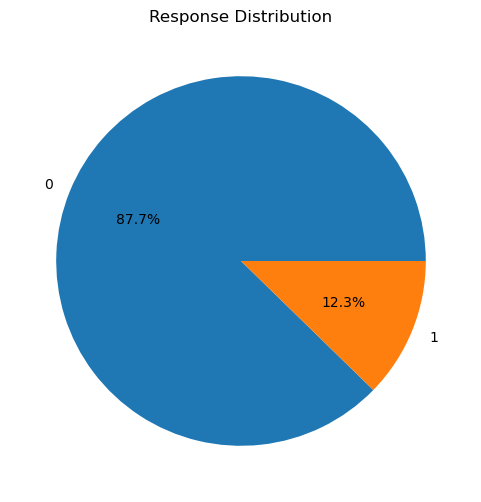
\includegraphics[width=\textwidth]{figures/response_distribution.png}
      \end{center}
    \end{column}
  \end{columns}
\end{frame}

% ── Slide 8: Univariate Distributions ────────────────────────────────────────
\begin{frame}{Feature Distributions}
  \begin{columns}[T]
    \begin{column}{0.24\textwidth}
      \textbf{Gender}
      \begin{itemize}\small
        \item Roughly balanced
        \item Probably not that useful on its own
      \end{itemize}
    \end{column}
    \begin{column}{0.24\textwidth}
      \textbf{Age}
      \begin{itemize}\small
        \item Skewed right
        \item Most customers are 20--50
        \item Tail goes up to 85
      \end{itemize}
    \end{column}
    \begin{column}{0.24\textwidth}
      \textbf{Vehicle Age}
      \begin{itemize}\small
        \item Most cars are 1--2 years old
        \item New cars ($<$1yr) almost never have damage
        \item Older cars $\to$ more damage
      \end{itemize}
    \end{column}
    \begin{column}{0.24\textwidth}
      \textbf{Annual Premium}
      \begin{itemize}\small
        \item Very skewed, lots of outliers
        \item Big spike at low premiums
        \item Clipped top 1\% for plots
      \end{itemize}
    \end{column}
  \end{columns}
\end{frame}

% ── Slide 9: Previously Insured ──────────────────────────────────────────────
\begin{frame}{Previously Insured: Strongest Predictor}
  \begin{columns}[T]
    \begin{column}{0.5\textwidth}
      \begin{itemize}
        \item If a customer already has vehicle insurance, they basically never respond
        \item Not insured: $\sim$22\% response rate
        \item Already insured: $\sim$0\% response rate
        \item This one feature pretty much determines the outcome
      \end{itemize}
    \end{column}
    \begin{column}{0.45\textwidth}
      \begin{center}
        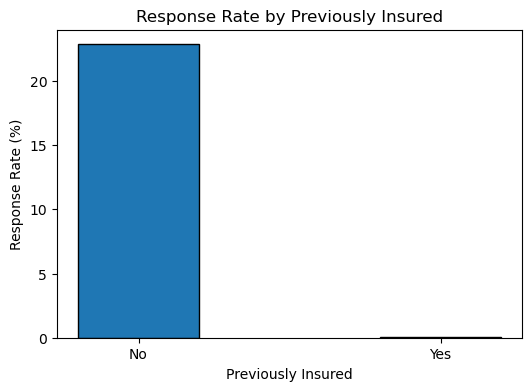
\includegraphics[width=\textwidth]{figures/previously_insured.png}
      \end{center}
    \end{column}
  \end{columns}
\end{frame}

% ── Slide 10: Vehicle Damage & Vehicle Age ───────────────────────────────────
\begin{frame}{Vehicle Damage \& Vehicle Age}
  \begin{columns}[T]
    \begin{column}{0.48\textwidth}
      \textbf{Vehicle Damage}
      \begin{itemize}
        \item Prior damage: response $\approx$ 24\%
        \item No damage: response $\approx$ 1\%
        \item Makes sense: if your car was damaged before, you probably want insurance
      \end{itemize}
    \end{column}
    \begin{column}{0.48\textwidth}
      \textbf{Vehicle Age}
      \begin{itemize}
        \item $<$1 year: low response
        \item 1--2 years: moderate
        \item $>$2 years: highest response
        \item Older car = more reason to get coverage
      \end{itemize}
    \end{column}
  \end{columns}
\end{frame}

% ── Slide 11: Response by Age Group ──────────────────────────────────────────
\begin{frame}{Response by Customer Age}
  \begin{columns}[T]
    \begin{column}{0.55\textwidth}
      \begin{itemize}
        \item Response rate is highest for ages 30--50
        \item Younger customers (20--29) are less interested even though there are lots of them
        \item 70+ also lower response
      \end{itemize}
    \end{column}
    \begin{column}{0.4\textwidth}
      \begin{center}
        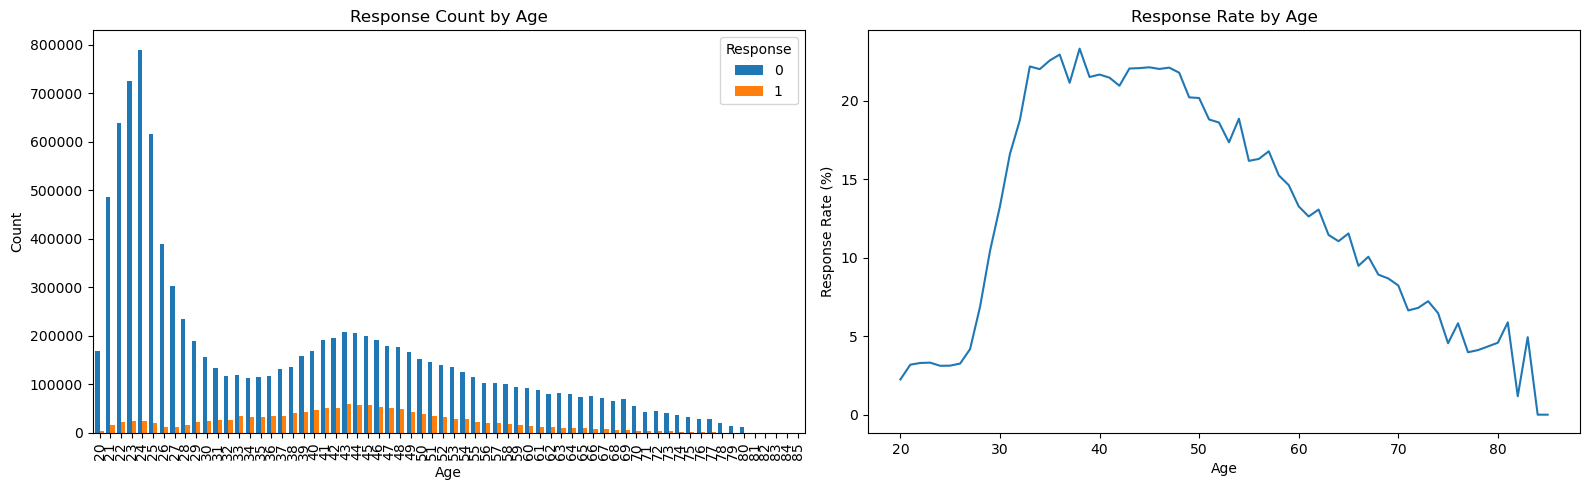
\includegraphics[width=\textwidth]{figures/response_by_age.png}
      \end{center}
    \end{column}
  \end{columns}
\end{frame}

% ── Slide 12: Sales Channel \& Region ────────────────────────────────────────
\begin{frame}{Sales Channel \& Region}
  \begin{columns}[T]
    \begin{column}{0.48\textwidth}
      \textbf{Policy Sales Channel}
      \begin{itemize}
        \item 152 distinct channels
        \item Response rate varies a lot across channels
        \item A few big channels dominate the volume
      \end{itemize}
    \end{column}
    \begin{column}{0.48\textwidth}
      \textbf{Region Code}
      \begin{itemize}
        \item 53 distinct regions
        \item Most cluster around $\sim$10\% response rate
        \item Some regions are quite different from the average
      \end{itemize}
    \end{column}
  \end{columns}
\end{frame}

% ── Slide 13: Annual Premium by Response ─────────────────────────────────────
\begin{frame}{Annual Premium by Response}
  \begin{columns}[T]
    \begin{column}{0.55\textwidth}
      \begin{itemize}
        \item Distributions overlap a lot between interested and not interested
        \item Medians are similar, so premium alone isn't a great predictor
        \item There's a spike at low premiums that tree models might pick up on
        \item Removed top 1\% outliers for the plot
      \end{itemize}
    \end{column}
    \begin{column}{0.4\textwidth}
      \begin{center}
        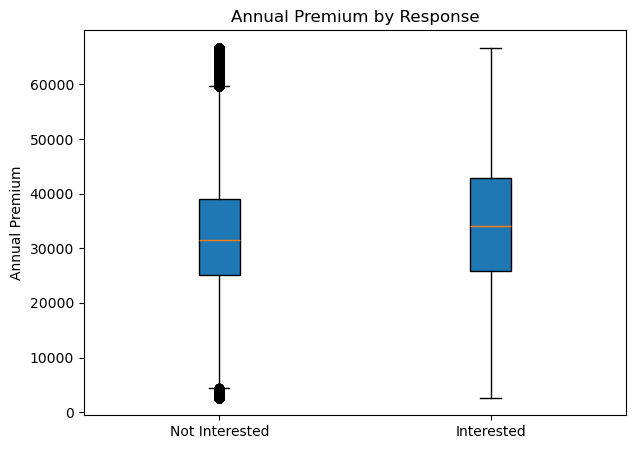
\includegraphics[width=\textwidth]{figures/annual_premium_response.png}
      \end{center}
    \end{column}
  \end{columns}
\end{frame}

% ── Slide 14: Correlation Heatmap ────────────────────────────────────────────
\begin{frame}{Correlation Analysis}
  Pearson correlation heatmap. Two pairs stand out:

  \vspace{0.3cm}
  \begin{table}[h]
    \centering
    \small
    \begin{tabular}{@{}lcc@{}}
      \toprule
      \textbf{Feature pair} & \textbf{$r$} & \textbf{What it means} \\
      \midrule
      \texttt{Previously\_Insured} \& \texttt{Vehicle\_Damage} & $-0.84$ & Almost the same info (inverted) \\
      \texttt{Age} \& \texttt{Vehicle\_Age} & $+0.78$ & Older customers tend to have older cars \\
      \bottomrule
    \end{tabular}
  \end{table}

  \vspace{0.3cm}
  Everything else is weakly correlated. These two pairs are what motivated the feature engineering experiment later.
\end{frame}

% ── Slide 15: Correlated Pairs, Closer Look ───────────────────────────────────
\begin{frame}{Correlation: Closer Look}
  \begin{columns}[T]
    \begin{column}{0.48\textwidth}
      \textbf{Previously Insured vs.\ Vehicle Damage} \\[0.2cm]
      $r \approx -0.84$
      \begin{itemize}
        \item Already insured $\Rightarrow$ almost never flagged as damaged
        \item They carry basically the same information (inverted)
        \item Could try dropping one of them
      \end{itemize}
    \end{column}
    \begin{column}{0.48\textwidth}
      \textbf{Age vs.\ Vehicle Age} \\[0.2cm]
      $r \approx +0.78$
      \begin{itemize}
        \item 20--29 age group: 97\% own cars $<$1 year
        \item Older groups: more spread out across vehicle ages
        \item This sharp break suggests trying an \texttt{Age $\times$ Vehicle\_Age} interaction
      \end{itemize}
    \end{column}
  \end{columns}
\end{frame}

% ── Slide 16: EDA Summary & Key Takeaways ───────────────────────────────────
\begin{frame}{EDA Summary}
  Main findings:
  \begin{itemize}
    \item Only 12.3\% positive, so we need to handle class imbalance
    \item \texttt{Previously\_Insured} is by far the strongest predictor
    \item \texttt{Vehicle\_Damage} is useful but almost redundant with it ($r = -0.84$)
    \item Older vehicles and ages 30--50 show higher response rates
    \item Sales channels vary a lot in conversion
    \item Two strong correlations suggest trying some feature engineering
  \end{itemize}
\end{frame}

% ══════════════════════════════════════════════════════════════════════════════
\section{Modelling}
% ══════════════════════════════════════════════════════════════════════════════

% ── Slide 17: Modelling Setup ────────────────────────────────────────────────
\begin{frame}{Modelling Setup}
  \begin{columns}[T]
    \begin{column}{0.48\textwidth}
      \textbf{Two models}
      \begin{itemize}
        \item \textbf{Logistic Regression} (linear baseline) \\
              {\small \texttt{class\_weight='balanced'}, standardised features}
        \item \textbf{LightGBM} (gradient-boosted trees) \\
              {\small \texttt{is\_unbalance=True}, 500 trees, lr $= 0.05$}
      \end{itemize}

      \vspace{0.4cm}
      \textbf{Two feature sets}
      \begin{itemize}
        \item \textbf{Original}: all 10 columns as-is
        \item \textbf{Engineered}: drop \texttt{Vehicle\_Damage}, frequency-encode
              \texttt{Region\_Code} \& \texttt{Policy\_Sales\_Channel},
              add \texttt{Age $\times$ Vehicle\_Age}
      \end{itemize}
    \end{column}
    \begin{column}{0.48\textwidth}
      \textbf{How I evaluated}
      \begin{itemize}
        \item 80/20 stratified split (same split for both feature sets)
        \item Main metric: ROC-AUC
        \item Also looked at Precision, Recall, F1 (threshold = 0.5)
      \end{itemize}

      \vspace{0.4cm}
      \textbf{Why the feature engineering}
      \begin{itemize}
        \item Motivated by the EDA correlations ($r=-0.84$, $r=+0.78$)
        \item Frequency maps computed on train split only (no leakage)
      \end{itemize}
    \end{column}
  \end{columns}
\end{frame}

% ── Slide 18: Results Comparison ─────────────────────────────────────────────
\begin{frame}{Results}
  \begin{table}[h]
    \centering
    \begin{tabular}{@{}lcccc@{}}
      \toprule
      \textbf{Model} & \textbf{ROC-AUC} & \textbf{Precision} & \textbf{Recall} & \textbf{F1} \\
      \midrule
      LR (original)          & 0.8365 & 0.2526 & 0.9801 & 0.4017 \\
      LR (engineered)        & 0.8222 & 0.2336 & 0.9739 & 0.3769 \\
      LightGBM (original)    & \textbf{0.8784} & 0.3000 & 0.9296 & 0.4536 \\
      LightGBM (engineered)  & 0.8693 & 0.2872 & 0.9255 & 0.4384 \\
      \bottomrule
    \end{tabular}
  \end{table}

  \vspace{0.3cm}
  \begin{itemize}
    \item LightGBM beats LR across the board
    \item Engineered features actually made things worse for both models
    \item Recall is high everywhere thanks to class weighting
    \item Precision is low because of the 88/12 imbalance (at threshold 0.5)
  \end{itemize}
\end{frame}

% ── Slide 19: Why Feature Engineering Didn't Help ────────────────────────────
\begin{frame}{Why Feature Engineering Didn't Help}
  \begin{enumerate}
    \item \textbf{Trees already handle this stuff} \\
          {\small LightGBM can learn non-linear splits, deal with high-cardinality features,
          and find interactions on its own, so the manual transforms were redundant.}

    \vspace{0.2cm}
    \item \textbf{Dropping \texttt{Vehicle\_Damage} lost some signal} \\
          {\small Even with $r \approx -0.84$ vs \texttt{Previously\_Insured}, the leftover
          information was still useful for some tree splits.}

    \vspace{0.2cm}
    \item \textbf{Frequency encoding threw away information} \\
          {\small Going from 53 distinct region codes to a single number lost the
          fine-grained differences between regions.}
  \end{enumerate}

  \vspace{0.3cm}
  Basically, feature engineering that helps linear models can actually hurt tree models
  that already handle these patterns internally.
\end{frame}

% ── Slide 20: Feature Importance ─────────────────────────────────────────────
\begin{frame}{Feature Importance}
  \begin{columns}[T]
    \begin{column}{0.48\textwidth}
      \textbf{Most important features (by gain)}
      \begin{enumerate}\small
        \item \texttt{Previously\_Insured}, way ahead of everything else
        \item \texttt{Vehicle\_Age}
        \item \texttt{Annual\_Premium}
        \item \texttt{Policy\_Sales\_Channel}
        \item \texttt{Region\_Code} / \texttt{Age}
      \end{enumerate}

      \vspace{0.3cm}
      Lines up well with what the EDA showed: \texttt{Previously\_Insured} dominates.
    \end{column}
    \begin{column}{0.48\textwidth}
      \begin{center}
        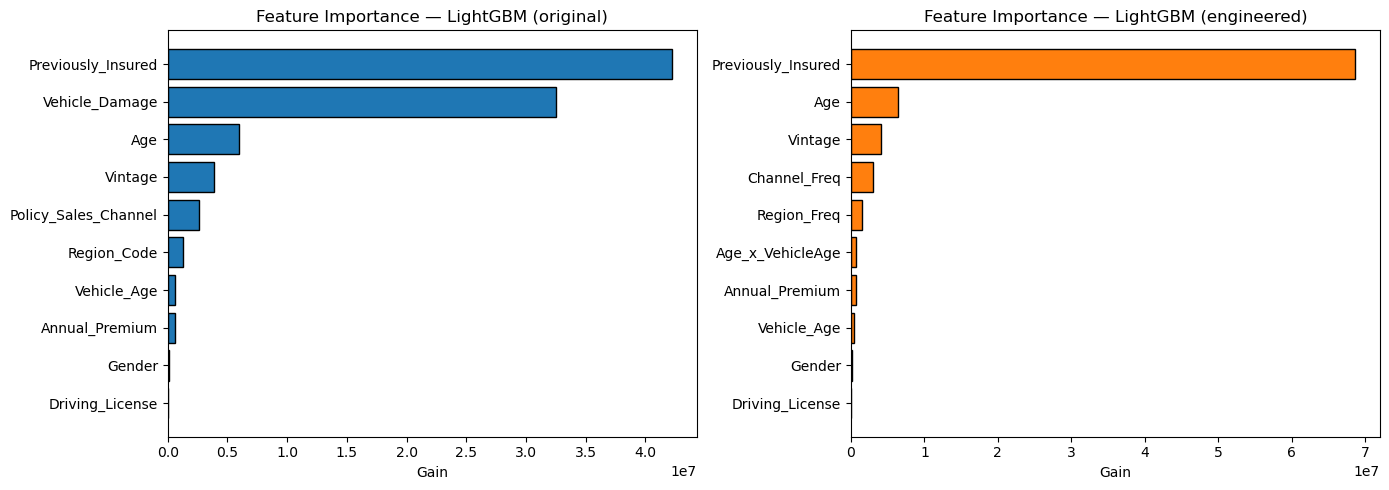
\includegraphics[width=\textwidth]{figures/feature_importance.png}
      \end{center}
    \end{column}
  \end{columns}
\end{frame}

% ── Slide 21: Conclusion & Limitations ──────────────────────────────────────
\begin{frame}{Conclusion \& Limitations}
  \textbf{What worked}
  \begin{itemize}
    \item LightGBM on original features was the best model (AUC = 0.878)
    \item Class weighting handled the imbalance well, with high recall across the board
    \item EDA findings were confirmed by the model (\texttt{Previously\_Insured} dominates)
  \end{itemize}

  \vspace{0.3cm}
  \textbf{What could be improved}
  \begin{itemize}
    \item Only used a single train/val split; k-fold would be more robust
    \item Didn't tune the classification threshold (just used 0.5)
    \item Could try other models like CatBoost or XGBoost
    \item Target encoding might work better than frequency encoding for high-cardinality features
  \end{itemize}
\end{frame}

\end{document}
